% EBMA paper for Political Analysis: As Accepted for Publication.



%\documentclass[pdftex,12pt,fullpage,oneside,endnotes]{amsart}
\documentclass[12pt,fullpage,endnotes]{article}
%\usepackage{apsr}
\usepackage{array,amsmath,psfrag,amssymb,subfigure,tabularx}
\usepackage{hyperref,multicol}
\usepackage{booktabs}
\usepackage[usenames]{color}
\usepackage{datetime}
\usepackage{dcolumn}
\usepackage{wrapfig}
\usepackage{setspace}
\usepackage{url}
\usepackage[english]{babel}
\usepackage{times}
\usepackage{multirow}
\usepackage[pdftex]{graphicx}
\usepackage{epstopdf}
\usepackage{lscape}
\usepackage{array}
\usepackage{booktabs}
\usepackage{hyperref}
\usepackage{endnotes}
\usepackage[top=3cm, bottom=3cm, left=2.3cm, right=2.3cm]{geometry} 
%\usepackage[nolist]{endfloat}

\newcommand{\note}[1]{\footnote{ #1 \vspace{4 mm}}}

\usepackage{natbib}
\bibpunct{(}{)}{;}{a}{}{,}
\bibdata{Bibliography_EBMA}
%\bibliographystyle{chicago}

\newboolean{blind}
\setboolean{blind}{false}


\title{Say yes to the guess: \\ Fitting quality ensembles on a tight
  (data) budget\thanks{This work was supported by the Information Processing Technology Office of the
    Defense Advanced Research Projects Agency through a
    holding grant is to the Lockheed Martin Corporation [FA8650-07-C-7749].}}
\author{
Jacob M. Montgomery\\
	Department of Political Science\\
	Washington University in St. Louis\\
	Campus Box 1063, One Brookings Drive\\
	St. Louis, MO, USA, 63130-4899 
	\and
Florian M. Hollenbach  \\
	Department of Political Science\\
	Duke University\\
	Perkins Hall 326 Box 90204\\
	Durham, NC, USA, 27707-4330
	\and
Michael D. Ward\\
	Department of Political Science\\
	Duke University\\
	Perkins Hall 326 Box 90204\\
	Durham, NC, USA, 27707-4330\\
	corresponding author: michael.d.ward@duke.edu
} 




\date{\today}


\begin{document}

\maketitle
\thispagestyle{empty}
\clearpage
\pagestyle{myheadings}
\markright{Montgomery, Hollenbach, \& Ward\hfill Ensemble BMA\hfill}
\newpage
%\singlespacing

\thispagestyle{empty}


\begin{abstract}
%\begin{doublespace}
 Bla bla blub
 %  \end{doublespace}
\end{abstract}

%\doublespacing
%\newpage


\setcounter{page}{1}

\section{Introduction}

Although accurate prediction of future events is not the primary goal
for most social sciences, recent years have witnessed spreading of
systematic forecasting from more traditional topics (e.g., GDP growth
and unemployment) to many new domains (e.g., elections and mass
killings) .  Several factors have motivated this increase.  To begin
with, testing systematic predictions about future events against
observed outcomes is generally seen as the most stringent validity
check of statistical and theoretical models.  In addition, forecasting
of important political, economic, and social events is of great
interest to policymakers and the general public who are generally less
interested testing theories of the world than correctly anticipating
and altering the future.

With the proliferation of forecasting efforts, however, comes a need
for sensible methods to aggregate and utilize the various scholarly
efforts.  One attractive solutions to this problem is to combine
various prediction models and create an ensemble forecast.  Combining
forecasts reduces reliance on any single data source or methodology,
but also allows for the incorporation of more information than any one
model is likely to include in isolation.  Across subject domains,
ensemble predictions are usually more accurate than any individual
component model. Second, they are significantly less likely to make
dramatically incorrect predictions \citep{Bates:1969, Armstrong:2001,
  Raftery:2005}.

The idea of ensemble learning itself has a long history in the machine
learning and nonparametric statistics community. The most thorough
treatment is found in \citet{Hastie:2009}. A wide range of statistical
approaches including neural nets, bagging, random forests, additive
regression trees, and boosting and more may be properly considered
ensemble approaches.  

One ensemble method advocated recently for forecasting is ensemble
Bayesian model averaging (EBMA). This methods was first proposed by
\citet{Raftery:2005} and recently forwarded as a useful method for the
social sciences by \citet{Montgomery:2012a}. In essence, EBMA creates a
finite mixture model that creates a kind of weighted average of
forecasts.  EBMA mixture models seek to collate the good parts of
existing forecasting models while avoiding over-fitting to past
observations or over-estimating our certainty about the future.  The
hope is for greater accuracy as both the knowledge and implied
uncertainty of a variety of approaches are integrated into a combined
predictive probability distribution.

However, there are several challenges for creating ensemble
predictions for many social science applications.  To begin with
amount and quality of data for calibrating ensembles is far from
ideal.  EBMA was first developed for use in weather forecasting where
measurement of outcomes is fairly precise and data is relatively
abundant.  Predicting, for instance, water surface temperatures in 200
locations across five days provides 1,000 observations by which model
weights can be calibrated.  Forecasting quarterly GDP
growth in the United States for five \textit{years} only provides 20.

A second and related issue is that there tends to be a lot more
forecasts than observations.  For example, the economic forecasting
survey has like a billion experts.  blah, balh

A final issue is the inconsistency with which forecasts are
issued. Given the lengthy time periods involved, of any given time
window there are many missing forecasts.  Moreover, we cannot assume
that forecasts for any time period from a specific model or team are
missing at random.  Particularly unsuccessful forecasts may be
suppressed.  Moreover, forecasts have tended to accumulate with more
observations being available for more proximate time periods.

One example of forecasting that combines all of these issues in the
prediction of U.S. Presidential elections.  Table 1 represents nearly
entirety of scholarly forecasts which produced more than one forecast
for elections in the 20th century \footnote{Citations.  Also something
  here about how we previously calibrated based on in-sample, but here
  we are focused on pure out-of-sample forecasts}.  In this instance
we have only five observations by which to calibrate a model while we
have nine forecasts.  Moreover, several of the individual forecasts
are missing for a significant portion of the data.  The forecast of
Cuzan, for instance, is missing for 60\% of the elections in the
dataset.

\begin{table}[ht]
\caption{Pre-election forecasts of the percent of the two-party vote going to the incumbent party in U.S. Presidential elections}
\footnotesize
\begin{center}
\begin{tabular}{rlrrrrrrrrr}
  \toprule
  & F & A & C & H & LBRT & L & Hol & EW & Cuz \\ 
  \midrule
  1992 & 55.7 & 46.3 & 49.7 & 48.9 & 47.3 &  &  &  &  \\ 
  1996 & 49.5 & 57.0 & 55.5 & 53.5 & 53.3 &  & 57.2 & 55.6 &  \\ 
  2000 & 50.8 & 53.2 & 52.8 & 54.8 & 55.4 & 60.3 & 60.3 & 55.2 &  \\ 
  2004 & 57.5 & 53.7 & 52.8 & 53.2 & 49.9 & 57.6 & 55.8 & 52.9 & 51.1 \\ 
  2008 & 48.1 & 45.7 & 52.7 & 48.5 & 43.4 & 41.8 & 44.3 & 47.8 & 47.7 \\ 
  \bottomrule

\end{tabular}
\end{center}
Forecasts were published prior to each election by \textbf{F}air, \textbf{A}bramowitz, \textbf{C}ampbell, \textbf{H}ibbs, \textbf{L}ewis-\textbf{B}eck and \textbf{R}ice (1992), Lewis-Beck and \textbf{T}ien  (1996-2008),   \textbf{L}ockerbie, \textbf{Hol}brook, \textbf{E}rikson and \textbf{W}lezien and \textbf{Cuz}an.  Data taken from CITE SILVER POST HERE.
\end{table}

While particularly egregious for presidential forecasting, these data
issues are endemic across the social sciences.  Blah, blah

In this paper, we explore several adjustments to the basic EBMA model
as specified in \citet{Montgomery:2012} that can help applied
researchers create ensemble forecasts even in the presence of these
kinds of data-quality issues.  Specifically, we show EBMA can be
adjusted to easily accomodate missing forecasts.  In addition, we
propose an alteration to the basic model.  Below, we briefly introduce
the basic EBMA model in Section \ref{model}.  We outline modifications
to the model for missingness and small samples in Sections
\ref{missing} and \ref{woc}. In Section \ref{empirics}, we apply the
adjusted EBMA model to unemployment data as well as presidential
forecasting models shown in Table 1.


\section{Notation and basic EBMA model} 
\label{model}

Assume a quantity of interest to forecast, $\mathbf{y}^{t^*}$, in some
future period $t^\ast \in T^\ast$.  Further assume that we have extant
forecasts for events $\mathbf{y}^t$ for some past period $t \in T$
that were generated from $K$ forecasting models or teams, $M_1, M_2,
\ldots, M_K$, for which have a prior probability distribution $M_k\sim
\pi(M_k)$. The PDF for $\mathbf{y}^t$ is denoted
$p(\mathbf{y}^t|M_k)$.  Under this model, the predictive PDF for the
quantity of interest is $p(\mathbf{y}^{t^*}|M_k$), the conditional
probability for each model is $p(M_k|\mathbf{y}^t) =
p(\mathbf{y}^t|M_k)\pi(M_k)/\underset{k=1}{\overset{K}{\sum}}p(\mathbf{y}^t|M_k)\pi(M_k)$
and the and the marginal predictive PDF is $p(\mathbf{y}^{t^*}) =
\underset{k=1}{\overset{K}{\sum}}
p(\mathbf{y}^{t^*}|M_k)p(M_k|\mathbf{y}^{t})$.  This can be viewed as
the weighted average of the component PDFs where the weights are
determined by each model's performance within the already-observed
period $T$.

\subsection{Dynamic ensemble forecasting}

The EBMA procedure assumes $K$ forecasting throughout the training
($T^{\prime}$) calibration ($T$) and test ($T^\ast$) periods.  The goal is
to estimate the parameters for the ensemble prediction model using
$\mathbf{f}^{t}_k$ for some period $T$.  It is then possible to
generate true ensemble forecasts ($\mathbf{f}_k^{t^\ast}$) for
observations in the test period $t^\ast \in T^*$.

Let $g_k(\mathbf{y}|\mathbf{f}_k^{s|t, t^\ast})$ represent the
predictive PDF of component $k$, which may be the original prediction
from the forecast model or the bias-corrected forecast.  The EBMA PDF
is then a finite mixture of the $K$ component PDFs, denoted
$p(\mathbf{y}|\mathbf{f}_1^{s|t}, \ldots,
\mathbf{f}_K^{s|t})=\overset{K}{\underset{k=1}{\sum}} w_k
g_k(\mathbf{y}|\mathbf{f}_k^{s|t})$, where $w_k \in [0,1]$ are model
probabilities, $p(M_k|\mathbf{y}^t)$, and $\sum_{k=1}^Kw_k=1$. The
ensemble predictive PDF with this notation is is then
$p(y|f_{1}^{t^\ast}, \ldots,
f_{K}^{t^\ast})=\overset{K}{\underset{k=1}{\sum}} w_k
g_k(y|f_{k}^{t^*})$.



Past applications have statistically post-process the predictions for
out-of-sample bias reduction and treat these adjusted predictions as a
component model. \citet{Raftery:2005} propose approximating the
conditional PDF as a normal distribution centered at a linear
transformation of the individual forecast,
$g_k(\mathbf{y}|\mathbf{f}_k^{s|t}) = N(a_{k0} +
a_{k1}\mathbf{f}_k^{t}, \sigma^2)$. However, in the presence of sparse
data, including the additional $\mathbf{a}$ parameters risks
over-fitting and reduced predictive performance.  We therefore use a
simpler formulation where $g_k(\mathbf{y}|\mathbf{f}_k^{t}) =
N(\mathbf{f}_k^{t}, \sigma^2)$.  Thus, the ultimate predictive
distribution for some observation $y^{t^\ast}$ is 

\begin{equation}
\label{pdf}p(y|f_1^{s|t^\ast},
\ldots, f_K^{s|t^\ast}) = \overset{K}{\underset{k=1}{\sum}} w_k
N(f_k^{t^\ast}, \sigma^2).
\end{equation}

\noindent This, is a mixture of $K$ normal distributions each of whose mean is
determined by $f_k^{t^\ast}$ and which is scaled by the model weights
$w_k$.

\subsection{Parameter estimation}

Since the component model forecasts, $f^t_1, \ldots, f^t_k$, are
pre-determined, EBMA model is fully specified by estimating model
weights, $w_1, \ldots, w_k$ and the common variance parameter
$\sigma^2$.  We estimate these by maximum likelihood methods
\citep{Raftery:2005}, although \citet{Vrugt:2008} have proposed
estimation via Markov chain Monte Carlo metods.  The log likelihood
function is

\begin{equation}
\mathcal{L}(w_1, \ldots, w_k, \sigma^2)=\sum_tlog\left(\sum_{k=1}^Kw_kN(f^t_k, \sigma^2) \right).
\end{equation}


\noindent This function cannot be maximized analytically, so
\citet{Raftery:2005} propose an EM algorithm which explicitly
expresses EBMA as a finite mixture model (CITE: McLachlan and Peel 200
and the new Imai AJPS).  We introduce the unobserved quantities
$z_k^t$, which represents the probabilty that observation $y^t$ is
``best'' predicted by model $k$.  The E step involves calculating
estimates for these unobserved quantities using the formula
\begin{equation}
\label{E-step}
\hat{z}^{(j+1)t}_{k} = \frac{\hat{w}^{(j)}_k
p^{(j)}(y|f_{k}^{t})}{\overset{K}{\underset{k=1}{\sum}}\hat{w}^{(j)}_kp^{(j)}(y|f_{k}^{t})},
\end{equation}
\noindent where the superscript $j$ refers to the $j$th iteration of
the EM algorithm.

$w_k^{(j)}$ is the estimate of $w_k$ in the $j$th iteration and
$p^{(j)}(.)$ is shown in \eqref{pdf}.  Assuming these estimates of
$z_{k}^{s|t}$ are correct, it is then straightforward to derive the
maximizing value for the model weights. Thus, the M step estimates
these as 

\begin{equation}
\label{M-step}
\hat{w}^{(j+1)}_k=\frac{1}{n}\underset{t}{\sum}\hat{z}^{(j+1)t}_{k},
\end{equation}

\noindent where $n$ represents the number of observations in the
validation dataset.  Finally,

\begin{equation}
\label{sigma}
\hat{\sigma}^{2(j+1)}=\frac{1}{n}\underset{t}{\sum}\overset{K}{\underset{k=1}{\sum}}\hat{z}^{(j+1)t}_{k}(y-f_{k}^{t})^2.
\end{equation}
\noindent The E and M steps are iterated until the improvement in the
log-likelihood is no larger than some pre-defined tolerance.  We
initiate the algorithm with the assumption that all models are equally
likely, $w_k = \frac{1}{K} ~ \forall ~ k \in [1, \ldots, K]$ and
$\sigma^2=1$.


\section{Missing forecasts}
\label{missing}

To accomodate missing ensemble values, \citep{Fraley:2010} modify the EM algorithm as follows. \footnote{In future versions of this paper, we hope to compare alternative methods for handling missing data including imputation gaussian copulas (CITATIONS). }  Define $$\mathcal{A}^t = \{i|\mbox{ensemble member i available at time t}\}.$$.

\noindent which is simply the indicators of the list of components that provide forecasts for observation $y_t$.   For convenience, define $\tilde{z}_k^{(j+1)t} \equiv {{\underset{k \in A^t}{\sum}}\hat{w}^{(j)}_kp^{(j)}(y|f_{k}^{t})}/{\underset{k \in A^t}\sum w_k^{(j)}}$.  Equation \ref{E-step} is then replaced with

\begin{equation}
\hat{z}^{(j+1)t}_{k} = \Bigg\{ \begin{array}{c} {\hat{w}^{(j)}_k p^{(j)}(y|f_{k}^{t})}/{\tilde{z}_k^{(j+1)t} } \mbox{ if } k \in \mathcal{A}^t\\ 0 \mbox{ if } k \notin \mathcal{A}^t \end{array}
\end{equation}



\noindent  The M steps in Equations \ref{M-step} and \ref{sigma} are likewise replaced with

\begin{equation}
\hat{w}^{(j+1)}_k=\frac{\underset{t}{\sum}\hat{z}^{(j+1)t}_{k}}{\underset{t}{\sum}\overset{K}{\underset{k=1}{ \sum}} \hat{z}_k^{(j+1)t}}
\end{equation}


\noindent and

\begin{equation}
\hat{\sigma}^{2(j+1)}=\frac{\underset{t}{\sum}\overset{K}{\underset{k=1}{\sum}}\hat{z}^{(j+1)t}_{k}(y-f_{k}^{t})^2 }{\underset{t}{\sum}\overset{K}{\underset{k=1}{ \sum}} \hat{z}_k^{(j+1)t}}.
\end{equation}


%\section{Window selection} Jacob thinks this should be a short subsection eventually.  But not for APSA.

\section{Small sample adjustment}
\label{woc}

When ensembles are calibrated on very few observations, there is an
increased chance that EBMA may over-weight high performing models in a
way that reduces out of sample performance.  Thus, we introduce a
``wisdom of crowds'' parameter, $c \in [0,1]$, that reflects our prior
belief that all models should receive some weight.  In essence, we
rescale $z^t_k$ to have a minimum value $\frac{c}{K}$.  This
essentially states that there is, at a minimum, a $\frac{c}{K}$
probability that the observation is correctly represented by each
model $k$.  Since $\overset{K}{\underset{k=1}{\sum}} z_k^t = 1$, this
implies that $z_k^t \in [\frac{c}{K}, (1-c)]$.  To achieve this, we
replace Equation \ref{M-step} above with

\begin{equation}
\hat{z}^{(j+1)t}_{k} = \frac{c}{K} + (1-c)\frac{\hat{w}^{(j)}_k
p^{(j)}(y|f_{k}^{t})}{\overset{K}{\underset{k=1}{\sum}}\hat{w}^{(j)}_kp^{(j)}(y|f_{k}^{t})}.
\end{equation}




Note that when $c=1$, that all models are considered equally
informative about the outcome and $w_k=\frac{1}{K} \forall K$. Thus, we see that the arithmetic mean or
median of component forecasts for time period $t$ represents a special
case of EBMA where $c=1$.\footnote{The mean or median would be
  equivalent depending on if the posterior mean or median is used to
  make a point prediction.}  Likewise, the general EBMA discussed in
\citet{Montgomery:2012} represents special case of this more general
model where $c=0$.

%\section{Simulations} Jacob think we will want just a bit of this.  But not for APSA.

\section{Applications}
\label{empirics}

Blah, blah transition paragraph here


\subsection{Quarterly unemployment}

Blah, blah.  Short lit review of this topic here.  We are looking at
predictions of U.S. unemployment four quarters out.

For each period $t$, we calibrate an ensemble model using forecaster
performance over the past ten quarters.  Only forecasts that had made
predictions for five of these quarters were included in the ensemble.
Thus, the EBMA model uses only 163 models out of a possible 293
forecasting models that made predictions during the period we study.
In addition to forecasts collected by the survey, we include the
``Green Book'' forecasts produced by the Federal reserve.  This model
serves both as a component of the ensemble and as a true baseline
model with which to compare the EBMA forecasts.  Due to missing data
early in the time series and the fact that Green Book forecasts are
sequestered for five years, we generate forecasts beginning in the
third quarter of 1983 and running through the fourth quarter of 2007.


Figure \ref{modelWeights} provides a visual representation of EBMA
model calibrations throughout this period.  In this figure, the wisdom
of crowds tuning parameter is set to a modest $c=0.05$.  The colors
indicate the model weight assigned to each component on a red-blue
color ramp (excluded components are simply blank).  In this figure
models assigned no weight are shown in dark blue while models that are
heavily weighted are shown in red.

\begin{figure}[h]
\caption{Clever caption here}
\label{modelWeights}
\begin{center}
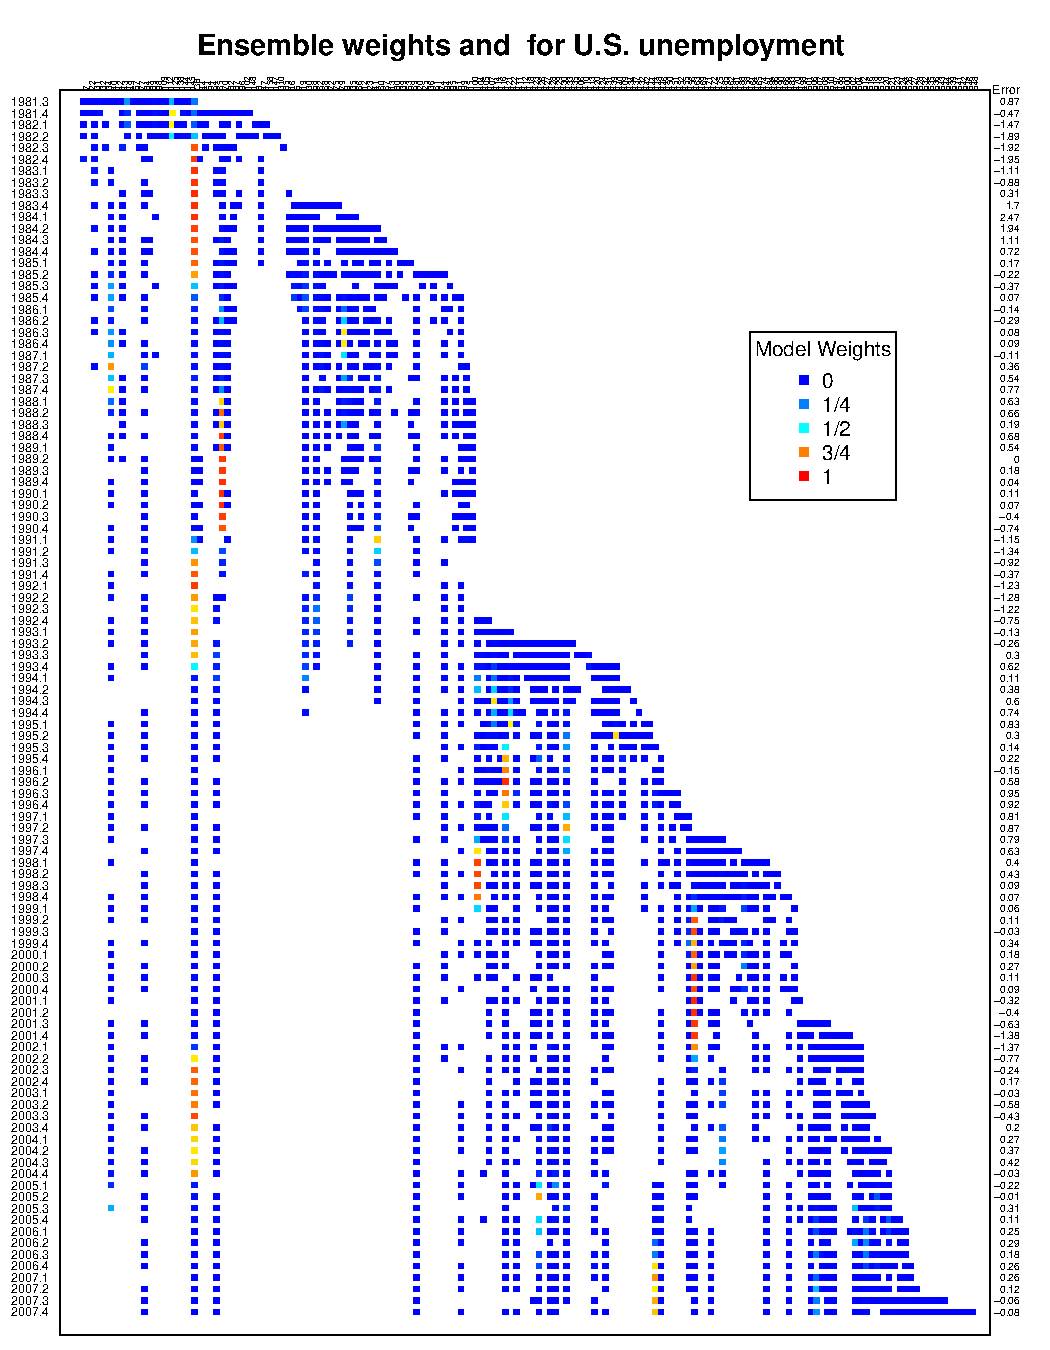
\includegraphics[scale=.95]{awesome}
\end{center}

\footnotesize Description of figure.

\end{figure}

Figure \ref{modelWeights} shows clearly difficulties inherent in
forecasting with this type of data.  For any given year, only a subset
of forecasting teams offer a prediction.  Further, an even smaller
subset both offer a predictions and have made a sufficiently large
number of prior forecasts to facilitate model calibration.  Finally,
the very sparseness of the data encourages the model to place a very
large amount of weight on the best performing models.

We now turn to evaluating the performance of the ensemble relative to
its 163 component forecasts.  To do this, we focus on eight model fit
indices available in the literature.  The eight metrics we use are
mean absolute error (MAE), root mean squared error (RMSE), median
absolute deviation (MAD), root mean squared logarithmic error (RMSLE),
mean absolute percentage error (MAPE), median absolute percentage
error (MEAPE), median relative absolute error (MRAE) and percent worse
(PW).  The latter two metrics are measured relative to a naive model
simply predicting the future rate of unemployment as being the same as
the current rate of unemployment.


\begin{figure}[h]
\caption{Clever caption here}
\label{compare2Components}
\begin{center}
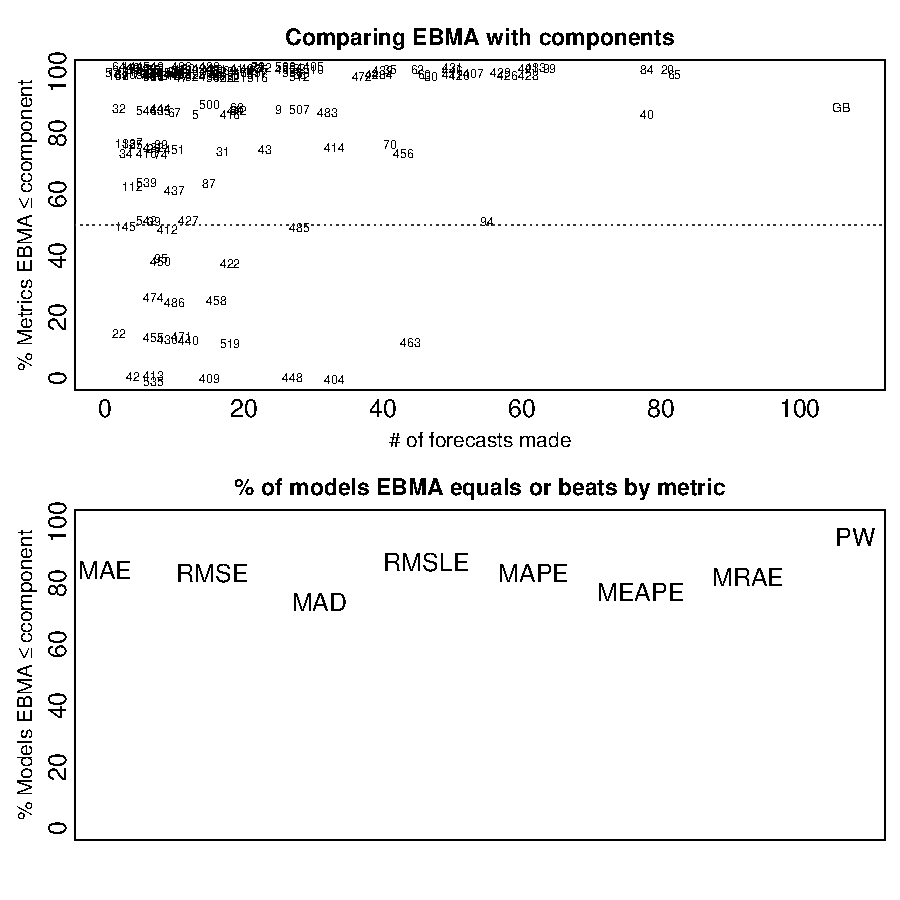
\includegraphics{compare2Components}
\end{center}
\end{figure}

It is important to note that many of these forecasters make
predictions in a relatively small subset of cases.  That is, the each
model $k$ offers forecasts for only a subset of cases $n_k \subset n$.
To create a fair comparison, therefore, we calculate these fit indices
only for $n_k \forall k \in [1,K]$.  By this measure, the EBMA model
performs very well.  Figure \ref{compare2Components} provides a
summary of these results.  The top panel shows the percentage of
metrics by which EBMA outperforms each component. The bottom panel
shows the percentage of component models that EBMA ``beats'' as
measured by each metric.

Notably, the relative superiority of EBMA to its components is
somewhat less for components that provide few forecasts.  This
reflects the fact that with so many forecasts, some are likely to be
more accurate than the ensemble by chance alone. However, across a
large number of forecasts, EBMA significantly outperforms any of its
components, including the Green Book (GB).  It is also worth noting
that only 6 out of the total 163 components outperforms EBMA on every
metric.

\begin{figure}[h]
\caption{Clever caption here}
\label{timeSeries}
\begin{center}
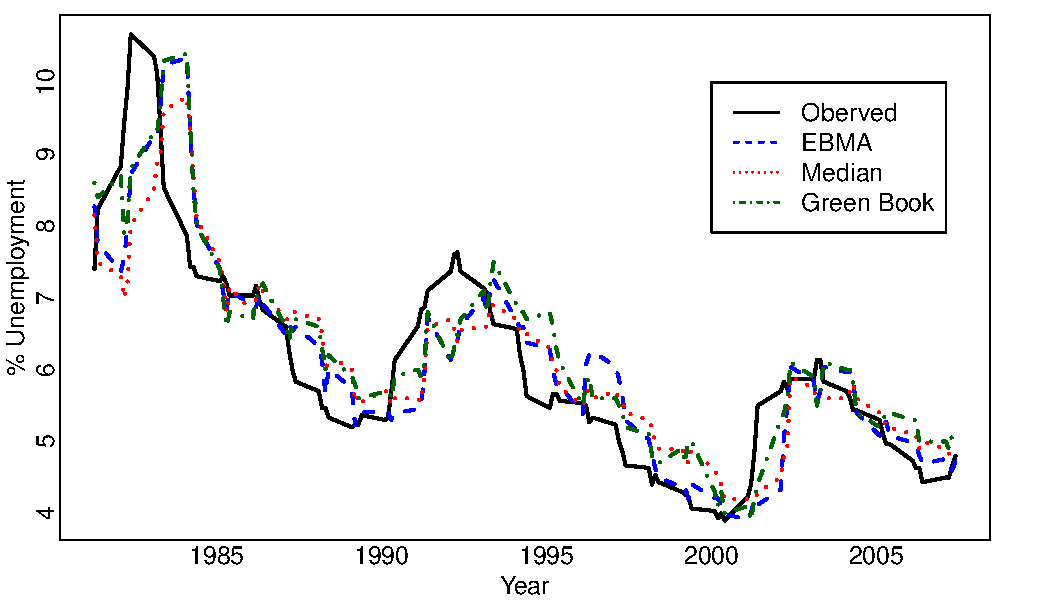
\includegraphics[scale=.8]{timeSeries}
\end{center}
\end{figure}


Another approach to evaluating the performance of EBMA is to compare
its predictive accuracy to that made by other systematic forecasting
efforts and methods of generating ensemble predictions.  Specifically,
we compare EBMA's predictive accuracy to (1) the Green Book, (2) the
median forecaster prediction and (3) the mean forecaster
prediction.\footnote{Note that the EBMA model is calculated only a the
  subset of forecasts that have made a sufficiently large number of
  recent predictions to calibrate model weights.  Thus, the median
  forecast and the ensemble forecast will not be the same even when
  $c=1$.  }  The first three of these forecasts and the true level of
unemployment are shown in Figure \ref{timeSeries}.

\begin{table}[h]
\caption{clever caption here}
\begin{center}
\begin{tabular}{lrrrrrrrr}
\toprule
 & MAE & RMSE & MAD & RMSLE & MAPE & MEAPE & MRAE & PW \\ 
\midrule
 EBMA (c=0)& 0.54 & 0.74 & 0.37 & 0.009 & 8.37 & 6.49 & \textbf{0.73} & \textbf{27.36} \\ 
  EBMA (c=0.05)& \textbf{0.54} & 0.74 &\textbf{ 0.37} & \textbf{0.009} & \textbf{8.33} & \textbf{6.30} & 0.75 & \textbf{27.36} \\ 
 EBMA (c=0.1)& 0.54 & 0.74 & 0.35 & 0.009 & 8.40 & 6.44 & 0.76 & 28.30 \\ 
EBMA (c=1) & 0.61 & 0.80 & 0.46 & 0.010 & 9.72 & 8.92 & 0.95 & 46.23 \\ 
 Green Book& 0.57 & \textbf{0.73} & 0.43 & 0.009 & 9.37 & 8.81 & 1.00 & 45.28 \\ 
 Forecast Median& 0.62 & 0.81 & 0.47 & 0.011 & 9.83 & 8.87 & 0.98 & 47.17 \\ 
Forecast Mean& 0.61 & 0.80 & 0.46 & 0.010 & 9.71 & 9.06 & 0.93 & 46.23 \\ 
\bottomrule
\end{tabular}
\end{center}

\label{compareTable1}
The model with the lowest score for each metric are shown in bold.  
\end{table}


Table \ref{compareTable1} compares these baseline models using all
eight of the metrics to EBMA moels with $c=$0, 0.05, 0.1, and 1
respectively.  The bolded cells in each column indicate the model that
performed ``best'' as measured by each metric.  With one exception,
the Green Book outperforms the ensemble by 0.01 on RMSE, EBMA model
outperforms both the Green Book forecast and unweighted mean and
median forecast.  Moreover, these results indicate that the $c$
parameter is best set to a smal number.  In general, the model with
$c=0.05$ performs best (or is tied for best) on six out of eight of
these metrics.


\subsection{U.S. presidential elections}

Informed by the above discussion, we return briefly to the example
with which we began -- predicting U.S. presidential elections.  Using
the forecasts shown in Table 1, we fit an EBMA model with $c=0.05$.
The model weights and in-sample fit statistics for the ensemble and
its components are shown in Table \ref{presModel}.

\begin{table}[ht]
\caption{The model names need to be fixed. Nice caption here.}
\label{presModel}
\begin{center}
\begin{tabular}{rrrr}
\toprule
 & W & RMSE& MAE\\ 
\midrule
EBMA &  & 1.92 & 1.56 \\ 
  Fair & 0.02 & 5.53 & 4.58 \\ 
  Abramowitz & 0.78 & 2.02 & 1.72 \\ 
  Campbell & 0.07 & 3.46 & 2.88 \\ 
  Hibbs & 0.04 & 2.68 & 2.44 \\ 
  LewisBeck & 0.06 & 2.78 & 2.28 \\ 
  Lockerbie & 0.00 & 7.33 & 6.97 \\ 
  Holbrook & 0.01 & 5.73 & 4.77 \\ 
  Erikson & 0.02 & 2.74 & 2.25 \\ 
  Cuzan & 0.00 & 0.99 & 0.75 \\ 
\bottomrule
\end{tabular}
\end{center}
\end{table}


Figure \ref{pres} shows the posterior predictive distribution for the
2008 election (top) and, based on current forecasts from each of the
component models, 2012 election.  We predict that Obama is going to
win by very little, but that our credible intervals are quite wide.

\begin{figure}[h]
\caption{Clever caption here}
\label{pres}
\begin{center}
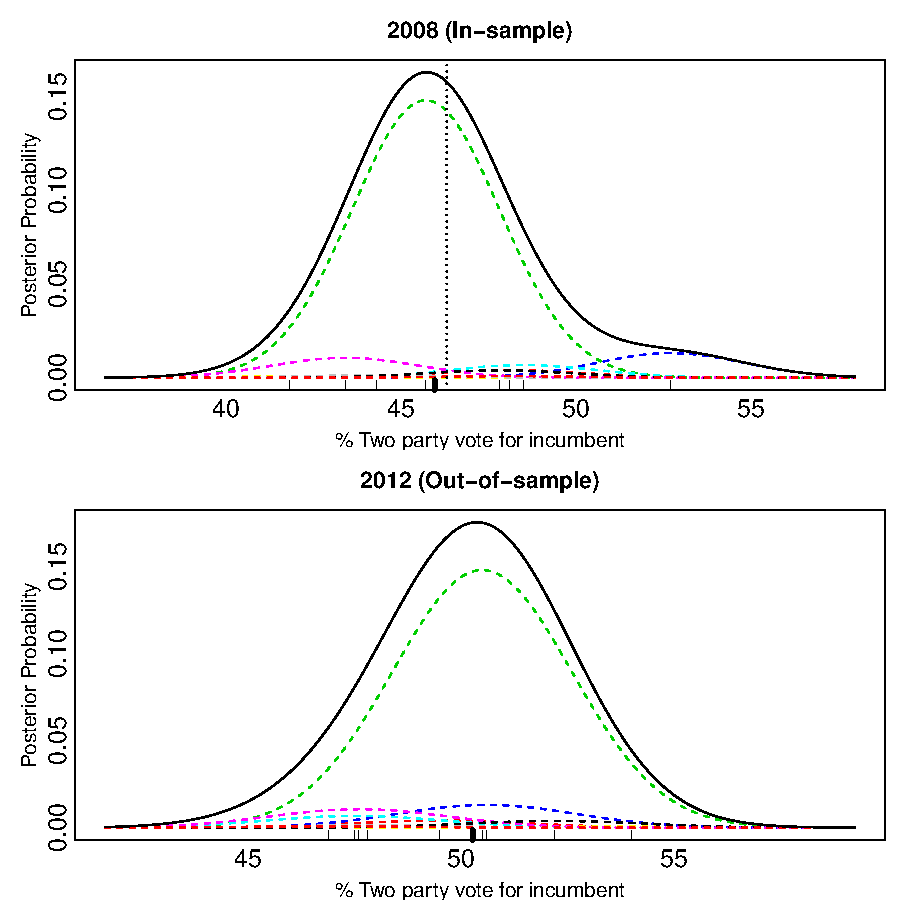
\includegraphics[scale=.8]{presForecast}
\end{center}

Explain the figure
\end{figure}





\section{Discussion} 


Super blah, blah.  We are awesome. Publish this article please.

In future drafts of this paper we hope to (1) compare alternative
methods of handling missing data (2) discuss how to select window of
time for calibration and (c) conduct some simulation studies to
explore settings for $c$ parameter and to test the numerical stability
of our results.



 \newpage
 \appendix


 \section*{Appendix}

Mathematical description of the various model fit statistics here.  


%%Bib 
\singlespacing
\bibliographystyle{apsr}
\bibliography{Bibliography_EBMA}


\end{document}
\bye
